\documentclass[conference]{IEEEtran}

% ---------- Paquetes recomendados ----------
\usepackage[utf8]{inputenc}  % Codificación UTF-8
\usepackage[T1]{fontenc}
\usepackage{graphicx}        % Para imágenes
\usepackage{amsmath, amssymb}
\usepackage{cite}            % Para referencias IEEE
\usepackage{url}             % Para URLs

% ---------- Inicio del documento ----------
\begin{document}

% ---------- Título ----------
\title{Búsqueda adversaria para aprender a jugar a Otelo}

\author{
    \IEEEauthorblockN{Eloy Sancho Cebrero}
    \IEEEauthorblockA{
        Universidad de Sevilla \\
        Sevilla, España \\
        elosanceb@alum.us.es
    }
    \and
    \IEEEauthorblockN{Iván Fernández Limárquez}
    \IEEEauthorblockA{
        Universidad de Sevilla \\
        Sevilla, España \\
        ivaferlim@alum.us.es
    }
}

\maketitle

% ---------- Resumen ----------
\begin{abstract}
Este trabajo presenta el desarrollo de un agente inteligente capaz de jugar al juego de Otelo (Reversi) mediante la integración de técnicas de búsqueda adversaria y aprendizaje automático. Concretamente, se ha implementado el algoritmo Monte Carlo Tree Search (MCTS) con el criterio de selección Upper Confidence Bound applied to Trees (UCT), junto con una red neuronal entrenada para evaluar estados de partida. El proceso de aprendizaje se basa en la autojugabilidad del agente, permitiendo generar y etiquetar automáticamente miles de posiciones de juego. Estas posiciones se utilizan para entrenar un modelo predictivo que sustituye a la función clásica de simulación en MCTS, mejorando así la toma de decisiones del agente. Se presenta también la arquitectura del sistema, la metodología de entrenamiento y un análisis de los resultados obtenidos. El objetivo principal es explorar, en un entorno simplificado, cómo la combinación de búsqueda y redes neuronales puede producir comportamientos estratégicos eficaces sin necesidad de funciones heurísticas manuales.
\end{abstract}

% ---------- Palabras clave ----------
\begin{IEEEkeywords}
Monte Carlo Tree Search, MCTS, Upper Confidence Bound for Trees, UCT, Othello, Otelo, Reversi, Python, Inteligencia Artificial, Red neuronal
\end{IEEEkeywords}

% ---------- Secciones ----------
\section{Introducción}
En muchos juegos podemos ver IA's que nos permiten jugar contra ellas \cite{russell2020}, ya sea como forma de introducirnos en el juego, o como maximo exponente del mismo.
Con el objetivo de aprender a crearlas, hemos creado una IA que aprende a jugar al juego de Otelo, para ello logramos crear un conjunto de datos con un
algoritmo base (Monte Carlo Tree Search, MCTS) y posteriormente usamos esos datos para entrenar una red neuronal implementada en ese mismo algoritmo que pudiera perfeccionar las jugadas a lo largo de la 
partida. En este documento estudiaremos como hemos logrado implementar todo esto, además de los resultados obtenidos al enfrentar la IA con red neuronal,
contra la que no tenia. Las principales dificultades al plantearnos esta tarea fueron, la elección de la estructura de la red neuronal y sus hiperparámetros, pues para
que la red mejorará había que elegir una tasa de aprendizaje efectiva y era imperativo el hacer una elección lógica de la arquitectura, puesto que hay numerosas
formas de montar una red neuronal y cada una tiene sus ventajas e inconvenientes para cada tarea. Ademas de esto, tambien planteo una ligera dificultad la funcion
de tree policy en el algoritmo de Montecarlo, pues era algo mas compleja que el resto.
\section{Preliminares}
Partimos de un agente que implementa montecarlo que se encarga de jugar partidas contra movimientos aleatorios, este guardará los estados intermedios 
en la partida y a cada uno se le asignará si, al acabar la partida, ganó, perdió o empató. Para representar estos estados hemos optado por hacer un csv, 
en el cual cada fila está formada de 65 elementos, los primeros 64 son el estado del tablero en orden, cada elemento es una casilla y si es 0 no hay nada,
si es 1 hay ficha blanca, si hay 2 hay ficha negra. El ultimo de los 65 elementos es la etiqueta que representa el resultado final de esa partida, propagado a cada estado intermedio,
-1 si perdió, 0 si empató, 1 si ganó. Tanto para enfrentarse a la IA como jugador, como para enfrentar a ambas IA entre sí, implementamos pygame, del cual se tratará su implementación mas adelante.
Para el diseño y entrenamiento de la red usamos tensorflow y keras, y para el tratamiento de datos empleamos mayoritariamente numpy, pues implementa muchas funciones utiles para presentar y amoldar
estos datos.

\section{Implementación}
Para la implementación del proyecto se han realizado los siguientes pasos: se ha creado una versión inicial de Otelo utilizando Pygame, se ha creado un agente básico utilizando el algoritmo de Monte Carlo Tree Search \cite{browne2012}, se han generado datos a partir de ese agente básico, se ha creado y, posteriormente, entrenado una red neuronal a partir de los datos generados, se ha utilizado la red neuronal como sustituta de una de las funciones de las que hace uso la implementación inicial del algoritmo MCTS y, finalmente, se ha adaptado la versión inicial de Otelo (en la que no se podía jugar contra ningún adversario) para que el agente desarrollado pudiese jugar contra el usuario.

A continuación, desarrollamos la implementación de cada uno de los pasos mencionados.

\subsection{Otelo en \texttt{pygame}}
El primer paso a seguir en la implementación del proyecto fue la creación del juego Otelo (sin presencia de un agente contra el que jugar) que nos serviría como base para crear tanto el agente MCTS como el agente final que haría uso de la red neuronal.

El juego se planteó como una matriz de ocho filas y ocho columnas en la que los jugadores realizan los cambios permitidos por las restricciones del reglamento de Otelo. En el contexto de Python, esta matriz se traduce como una lista que contiene ocho listas que, a su vez, contienen ocho números cada una y representan las ocho filas en las que se divide el tablero, siendo cada número almacenado en esa lista de listas la representación de lo que hay en cada casilla (no hay ficha, una ficha blanca o una ficha negra), haciendo un total de sesenta y cuatro números. En esta implementación de Otelo sólo hay tres posibles números que representan el color de la ficha que hay en cada casilla del tablero, el resultado final de la partida y, adicionalmente, se utilizan también para saber el turno actual de una partida en curso. Estos números son: el cero (no hay ficha en la casilla o el juego ha terminado en empate), el uno (hay una ficha blanca en una casilla, el jugador de las blancas ha ganado la partida o es el turno de dicho jugador) y el dos (hay una ficha negra en la casilla, el jugador de las blancas ha ganado la partida o es el turno de dicho jugador).

Sin embargo, esta lógica es la base que hay detrás de la interfaz gráfica mediante la cual una persona puede jugar a esta implementación de Otelo, una interfaz gráfica creada gracias a los recursos de la librería Pygame. Si bien es cierto que, entre las alternativas posibles para la implementación de este juego estaba la opción de crear un script que permitiera jugar a Otelo mediante texto (es decir, representando directamente la lógica que se ha mencionado anteriormente), valoramos más la opción de hacer uso de la librería Pygame, pues no sólo el juego sería mejor desde el punto de vista visual (aunque, dentro de los mínimos a cumplir en el proyecto, no desde el punto de vista técnico), sino que también se concibió el uso de Pygame como una manera muy intuitiva de empezar la implementación del proyecto partiendo desde cero.

Se construyó el script \texttt{otelo.py} para que, al ser ejecutado, inicializase una pantalla de 640 píxeles de alto y ancho en la que el color de fondo es el verde y varias líneas negras dividen las casillas cuadradas de 80 píxeles de lado. Adicionalmente, se representan las fichas como círculos blancos o negros de diámetro un poco menor al lado de las casillas y de centro situado en el centro de la casilla en la que está cada uno. Este script, como todos los videojuegos creados a partir de Pygame, contiene un bucle principal que comprueba si el usuario ha cerrado la ventana, comprueba si el usuario ha hecho clic en alguna casilla, etc. En este bucle, dentro de la implementación inicial que se trata en este apartado, sencillamente se comprueba en qué lugares de la pantalla el usuario hace clic para colocar la ficha correspondiente (en caso de que la disposición del tablero lo permita) y se alternan los turnos (\texttt{turno = 1} y \texttt{turno = 2}). Cada vez que ocurre esto, se pinta el tablero en base a la nueva matriz que lo representa y que contiene los cambios provocados por la acción del jugador (tanto la posición de la nueva ficha colocada como las fichas volteadas).

El proceso para hacer esto consiste en lo siguiente: primero es necesario convertir el píxel en el que el usuario ha hecho clic en una casilla. Para ello, se hace una división entera de cada coordenada del píxel entre la longitud en píxeles de cada casilla. Posteriormente, teniendo las coordenadas de la casilla, se comprueba si es posible colocar ficha en la casilla seleccionada. Si no lo es, no ocurre nada, pero si lo es, se coloca la ficha en la casilla y se voltean las fichas que deberán darse la vuelta tras la aparición de la nueva ficha. Para realizar tanto la comprobación de movimientos disponibles como el volteo de las fichas, se utilizan funciones que comprueban si existen fichas que serán volteadas tras la colocación de la nueva ficha (aunque, anteriormente, se comprueba si la matriz contiene un cero en el lugar seleccionado) y se guardan las coordenadas de dichas fichas para, en la modificación del tablero previa al cambio de turno, cambiar el color de las fichas a voltear; en caso de que el turno actual sea igual a 1 (blancas) se asigna el valor 1 a las celdas de la matriz equivalentes a las casillas afectadas y en caso de que el turno actual sea el del jugador de las fichas negras (igual a 2), se hace exactamente lo mismo pero asignando un 2 a las celdas correspondientes.

Por último, es necesario recalcar varios puntos: primero, antes del proceso anteriormente descrito, se comprueba si el jugador tiene movimientos disponibles. Si no los tiene, se cambia el turno. Segundo (como ya se ha mencionado) en esta implementación no existe ningún agente, el usuario coloca fichas tanto para el jugador de las blancas como para el jugador de las negras. Y tercero, es necesario recalcar que todo lo explicado es fundamental para el desarrollo del agente MCTS, pues implementan la lógica que seguirá el agente para poder jugar correctamente a Otelo.

\subsection{Motor MCTS con UCT}
Tras la implementación del juego base, se procedió a crear el que denominamos "Motor MCTS", que no es más que el algoritmo de Monte Carlo Tree Search adaptado a juego de Otelo (junto con sus funciones auxiliares) que utilizará el agente básico para poder jugar partidas y guardar los datos recogidos durante dichas partidas.

Para crear este motor de la forma más eficiente, fue necesario hacer uso de Python orientado a objetos (en otras palabras, fue necesaria la creación de una clase en Python). La clase creada es la clase \texttt{Nodo}. Esta clase es fundamental para el correcto funcionamiento del algoritmo, pues el algoritmo MCTS es simplemente un método para llevar a cabo la denominada "Búsqueda adversaria" (como lo es también el algoritmo Minimax alfa-beta) en la que creamos un árbol en el que los nodos son los estados en los que se encuentra la partida del juego en cada momento y las acciones llevadas a cabo partiendo de cada estado llevan a los distintos hijos de cada nodo, si los hay. La clase \texttt{Nodo} almacena los siguientes atributos:

\begin{itemize}
    \item \textbf{Estado}. Almacena la disposición del tablero y es lo que, en esencia, representa el nodo en cuestión.
    \item \textbf{Turno}. Almacena simplemente el turno del jugador que puede colocar ficha.
    \item \textbf{Padre}. Almacena un objeto de tipo \texttt{Nodo} que representa el nodo padre del nodo en cuestión. Por defecto, su valor es nulo.
    \item \textbf{Hijos}. Almacena una lista de objetos de tipo nodo que representa el conjunto de hijos del nodo en cuestión. A pesar de que en esta implementación ese conjunto de hijos se trata como una lista, el orden de los hijos no es realmente relevante a nivel conceptual. El valor asignado inicialmente es una lista vacía.
    \item \textbf{N}. Almacena el número de veces que el nodo ha sido visitado por las partidas simuladas. El valor asignado inicialmente es 0.
    \item \textbf{Q}. Almacena la recompensa acumulada de todas las partidas simuladas que han visitado el nodo en cuestión. El valor asignado inicialmente es 0.
    \item \textbf{Movimientos por hacer}. Almacena el conjunto de movimientos representados mediante la tupla \texttt{(fila, columna)}, disponibles para el jugador que puede colocar ficha (según el atributo \texttt{turno}). Es perfectamente posible que el jugador no tenga movimientos disponibles y que la lista esté vacía. Este atributo siempre se inicializa mediante la función \texttt{movimientos\_disponibles}, que devuelve el conjunto de jugadas válidas a partir del estado del tablero (atributo \texttt{estado}) y el turno actual (atributo \texttt{turno}).
    \item \textbf{Movimiento}. Almacena el movimiento representado mediante la tupla \texttt{(fila, columna)} que ha dado lugar al estado del nodo en cuestión. Este movimiento es nulo en el estado inicial de la partida, ya que no se ha realizado ninguna jugada previa. Por ello, su valor por defecto es \texttt{None}, y solo se especifica si el nodo representa un estado generado a partir de una jugada anterior.
\end{itemize}

Por otro lado, tenemos la función principal \texttt{mcts}, que se encarga de llevar a cabo los pasos indicados por el algoritmo MCTS. Primero crea un árbol con un nodo raíz a partir del tablero y el turno dados como parámetros. Posteriormente, realiza un número determinado de iteraciones (50 por defecto, aunque es posible pasar como parámetro otro número) y en cada iteración crea un nodo hijo a partir de la función \texttt{tree\_policy}, realiza una simulación de la partida a partir de ese nodo (mediante la función \texttt{defaut\_policy}) y retropropaga la recompensa obtenida al final de la partida simulada por el nodo y por el raíz (el nodo padre). Finalmente, tras las iteraciones especificadas, la función escoge el mejor movimiento de entre los movimientos disponibles para el nodo raíz.

La función \texttt{tree\_policy} que utiliza nuestra implementación del algoritmo MCTS se encarga de añadir a la lista de \texttt{hijos} del nodo raíz todos sus hijos (es decir, se encarga de expandir totalmente el nodo) y escoger el mejor hijo de todos, basándose en la ecuación del algoritmo Upper Confidence Bound for Trees. Para ello, recorre la lista de movimientos por hacer del nodo raíz y realiza las expansiones pertinentes utilizando la función \texttt{expand}. Esta función, dado el nodo raíz, simplemente elimina uno de los movimientos restantes de su lista de movimientos por hacer y crea el nodo que se formará a partir de la realización del movimiento especificado por la acción borrada de la lista ya mencionada (añadiendo también dicho nodo a la lista de \texttt{hijos} del nodo padre).

Una vez expandido por completo el nodo, se elige el mejor hijo mediante la función \texttt{mejor\_hijo}. Esta función, que se fundamenta en la ecuación UCT, calcula el resultado de la ecuación~\eqref{eq:uct} para cada uno de los hijos que hay en la lista de del nodo padre.

Una vez expandido por completo el nodo, se elige el mejor hijo mediante la función \texttt{mejorhijo}. Esta función, que se fundamenta en la ecuación UCT, calcula el resultado de la ecuación~\eqref{eq:uct} para cada uno de los hijos que hay en la lista de del nodo padre.

\begin{equation}
UCT = \frac{Q(v')}{N(v')} + C \cdot \sqrt{\frac{2 \cdot \ln N(v)}{N(v')}}
\label{eq:uct}
\end{equation}

\begin{itemize}
    \item $Q(v')$: recompensa acumulada del nodo hijo v'.
    \item $N(v')$: número de veces que se ha visitado el nodo hijo.
    \item $N(v)$: número de veces que se ha visitado el nodo padre v.
    \item $C$: constante de exploración que determina la importancia que le damos a explorar nodos poco visitados frente a explotar los nodos que han sido visitados bastantes veces y que son conocidos como nodos que suelen llevar a la victoria. En nuestro caso, hemos declarado el valor por defecto de $C$ en la función \texttt{mejor\_hijo} como $\sqrt{2}$ basándonos en lo indicado por los autores del artículo original de UCT. Sin embargo, es necesario tener en cuenta que el mejor valor para esta constante no tiene por qué ser este valor y que depende mucho de las circunstancias concretas del juego en cuestión.
\end{itemize}

Una vez expandido por completo el nodo raíz y escogido su mejor hijo, pasamos al funcionamiento de la función \texttt{default\_policy}. Esta función, siguiendo rigurosamente el pseudocódigo escrito en el artículo "A survey of Monte Carlo Tree Search Methods", realiza una simulación completa partiendo desde el nodo elegido como mejor hijo del raíz hasta el final de la partida, devolviendo una recompensa en función del resultado de la partida: -1 para derrotas, 0 para empates y +1 para victorias. Para realizar esta simulación, esta función no sigue construyendo el árbol realmente, se limita a elegir una acción aleatoria de la lista de acciones disponibles dado un tablero (o estado) y un turno, realiza los cambios pertinentes en el tablero y cambia de turno. Este proceso es repetido hasta que se detecta que el estado es terminal gracias a la función \texttt{no\_terminal} (función también usada en otras funciones anteriormente mencionadas). Esta función sólo comprueba que hay movimientos disponibles tanto en el turno actual como en el turno siguiente, en caso contrario, se determina que la partida ha llegado a su fin.

Tras la simulación y la obtención de la etiqueta correspondiente (-1, 0 ó 1), se retropropaga la recompensa tanto por el nodo hijo como por el nodo padre (el raíz). Para retropropagar la recompensa, realiza los siguientes cambios en los atributos \texttt{n} y \texttt{q} de cada nodo:

\begin{itemize}
    \item Para \texttt{n}: se guarda el valor \texttt{n} + 1.
    \item Para \texttt{q}: se guarda el valor \texttt{q} + $\Delta$, siendo $\Delta$ la recompensa obtenida a partir de la partida simulada por \texttt{default\_policy}
\end{itemize}

Por último, tras la realización de todas las iteraciones indicadas a la función \texttt{mcts}, se elige la mejor acción de entre todas las posibles, eligiendo el mejor hijo del nodo raíz y devolviendo el atributo \texttt{movimiento} que, como se ha mencionado anteriormente, indica el movimiento que ha dado lugar al estado del tablero que representa dicho nodo.

\subsection{Agente básico generador de datos}
El agente básico generador de datos es el agente que hace uso de lo que hemos denominado "motor MCTS" para jugar partidas y registrar todos y cada uno de los estados en los que el tablero se ha encontrado durante cada una de las partidas generadas. Cabe recalcar que, todavía, no es posible jugar contra este agente y el juego de Otelo implementado sigue siendo la básica versión en el que el único jugador existente es el usuario y éste alterna entre el control de las fichas blancas y las negras.

Este agente se limita a jugar partidas contra un adversario que elige acciones aleatorias y registra en un archivo llamado \texttt{datos\_otelo.csv} todos los estados del tablero en cada una de las partidas jugadas. Es posible indicar a la gente lo siguiente: el número de partidas a realizar, el jugador que utilizará el algoritmo MCTS y el número de iteraciones que realizará dicho algoritmo. Para cada partida, se siguen los siguientes pasos:

\begin{enumerate}
    \item Se inicializan el tablero de apertura, el turno inicial (\texttt{turno = 2}), correspondiente al jugador de las negras) y un historial (una lista vacía) que registrará todos los estados por los que pasará el tablero durante la partida.
    \item Se inicializa un bucle que repetirá lo siguiente mientras el estado en el que nos encontremos no sea un estado terminal: se añade el estado actual del tablero al historial de estados y se procede a realizar un movimiento según el turno en el que nos encontremos.
    \begin{enumerate}
        \item Turno del agente MCTS: se elige un movimiento en función de lo indicado por el algoritmo MCTS. Si no hay movimientos disponibles se pasa turno.
        \item Turno del rival: se elige un movimiento aleatorio. Si no hay movimientos disponibles, se pasa turno.
	    \item En caso de que haya habido movimiento disponible para el jugador en cuestión, se coloca la ficha en el lugar indicado y se voltean las fichas afectadas por la colocación de la nueva ficha. Posteriormente, se pasa turno.
    \end{enumerate}
    \item Tras llegar a un estado detectado como terminal, se finaliza el bucle y se añade el estado final al historial de estados.
    \item Se evalúa el resultado de la partida. Si el jugador indicado como parámetro al agente tiene más fichas en el tablero que su oponente, se guarda el valor \texttt{1}, si ocurre lo contrario se guarda el valor \texttt{-1} y si ninguno de los jugadores tiene más fichas que el otro se guarda el valor \texttt{0}.
    \item Adicionalmente, se muestran en la consola datos como el estado final del tablero, la cantidad de fichas de cada jugador, etc.
    \item Para cada uno de los estados guardados en el historial, se realiza lo siguiente:
    \begin{enumerate}
        \item Se convierte el estado a una fila de 64 números, definiendo cada número lo que hay en su correspondiente casilla dentro del tablero.
        \item Se añade a la fila un número adicional, la recompensa obtenida en el paso \textbf{4.}
	    \item Se escribe la fila en el archivo mencionado al principio de este apartado.
    \end{enumerate}
\end{enumerate}

Finalmente, tras jugar todas las partidas indicadas, se guarda el archivo \texttt{datos\_otelo.csv} en la ruta especificada al agente. Dicho archivo contiene, en orden, todos los estados intermedios de todas las partidas jugadas, siendo posible observar la cantidad de veces que el jugador que utilizó MCTS perdió y cuántas veces dicho jugador ganó o, por lo menos, empató. Esos datos, como se explicará a continuación, serán utilizados para el entrenamiento de la red neuronal que sustituirá la elección aleatoria de movimientos en la función \texttt{default\_policy} del motor MCTS.

\subsection{Diseño de la red neuronal}
La red neuronal como se mencionó en la introduccion esta hecha con keras, para hacerla 
creamos un input de la forma (8,8,2) lo que significa que tomaremos un tablero de 8x8 casillas y cada casilla
sera un canal doble, esto no es mas que una lista con dos valores binarios, si ambos son 0 la casilla estará vacía
si el primero es 1, la casilla estará ocupada por una ficha blanca, si el segundo es 1 entonces hay una ficha negra.


Se hace de esta forma puesto que, de esta manera la red no deberá "adivinar" que el valor 2 es para las negras y el 1 para las blancas
de otra forma la red podría interpretar que, por ejemplo, 2 es "mejor" que 1, entre otras complicaciones.
Así pues la red neuronal se compone de varias capas:
\begin{itemize}
    \item \textbf{Capa de entrada}: Se encarga de tomar los datos de entrada, el input ya ha sido explicado 
    \item \textbf{Capas convolucionales}: Las primeras capas de la red neuronal son de tipo convolucional y utilizan filtros de tamaño $3 \times 3$. Estas capas se inspiran en el funcionamiento de las redes convolucionales tradicionales aplicadas al procesamiento de imágenes, adaptadas aquí al tablero de Otelo, representado como una matriz de dimensiones $8 \times 8$ con dos canales.

Cada filtro o \textit{kernel} o informalmente hablando \textit{"plantilla"} convolucional actúa como una ventana entrenable que recorre la matriz de entrada y busca patrones locales que puedan ser relevantes para la toma de decisiones del agente. Matemáticamente, un filtro de tamaño $3 \times 3$ posee un conjunto de nueve pesos (uno por cada celda del filtro), y su aplicación sobre una subregión del tablero consiste en realizar una operación de convolución: multiplicar cada uno de esos pesos por el valor correspondiente de la celda del tablero en la que se superpone, y sumar todos los productos obtenidos. Esta suma constituye un único valor de salida que representa la "respuesta" del filtro ante dicha subregión.

Este proceso se repite a lo largo de toda la matriz de entrada, desplazando el filtro sobre cada posible submatriz $3 \times 3$ del tablero. Como resultado, se genera un nuevo mapa de activación (o tablero de salida) que contiene, en cada posición, el valor calculado mediante la operación descrita. Este mapa o "nuevo tablero" representa una transformación intermedia de los datos de entrada que representan ciertos patrones en el juego, como columnas de fichas, filas de fichas negras, casillas vacías...

 Al aplicar un filtro, la posición central de la región sobre la que se aplicó el mismo pasa a ser el nuevo valor en la "celda" del mapa de salida. Así que como cada capa convolucional va recibiendo "tableros" enteros con identificaciones de patrones de la anterior, a cada capa los patrones detectados son mas abstractos. Lo que se podría traducir a un "entendimiento" mas profundo del juego, o a la posibilidad de visualizar jugadas mas estratégicas por parte del agente
\item \textbf{Capa de aplanado}: Esta capa transforma los tableros (tensores tridimensionales, $8 \times 8 \times 128$) generados por la última capa convolucional en un vector unidimensional. Esta operación permite conectar las capas convolucionales, que trabajan sobre estructuras espaciales, con las capas densas posteriores, que operan sobre vectores. En nuestro caso, el resultado es un vector de 8192 elementos.

\item \textbf{Capa de desactivación (\texttt{Dropout})}: Se introduce una capa \texttt{Dropout} con una tasa de desactivación del 50\,\% para reducir el riesgo de sobreajuste. Durante el entrenamiento, esta capa apaga aleatoriamente la mitad de las neuronas que alimentan la siguiente capa. Al estar apagadas su output no se generará y por ende el ajuste será mas acotado.

\item \textbf{Capa densa}: A continuación, se emplea una capa totalmente conectada (\texttt{Dense}) que reduce los 8192 valores obtenidos tras el aplanado a una representación más compacta de 256 dimensiones. Estos valores pueden interpretarse como una codificación intermedia que captura la cantidad y relevancia de ciertos patrones estratégicos en el estado actual del tablero.

\item \textbf{Capa de salida}: Finalmente, se utiliza una capa densa con una única neurona y función de activación tangente hiperbólica (\texttt{tanh}), que produce una salida en el rango $[-1, 1]$. Este valor representa una estimación de lo favorable o desfavorable que es una determinada posición para el jugador actual.

    \item \textbf{Optimizador y función de pérdida}: Para la optimización del modelo se ha utilizado el algoritmo \texttt{Adam} (Adaptive Moment Estimation), ampliamente empleado en redes neuronales profundas. Este optimizador ajusta de forma adaptativa las tasas de aprendizaje de cada parámetro, lo cual resulta especialmente útil en escenarios con estructuras complejas como las redes convolucionales. En cuanto a la función de pérdida, se ha empleado el error cuadrático medio (\texttt{MSE}), ya que el objetivo de la red es aproximar una evaluación numérica continua del estado del juego en el intervalo $[-1, 1]$.
\end{itemize}


\subsection{Entrenamiento de la red neuronal}

El proceso de entrenamiento de la red neuronal se llevó a cabo utilizando inicialmente los datos generados por el agente MCTS básico. Una vez entrenado un primer modelo de la red, se implantó dicho modelo dentro del agente MCTS para generar nuevas partidas con decisiones guiadas por la red neuronal. Esta estrategia permite obtener estados de juego más sofisticados, al incorporar en la generación de datos conocimiento previamente aprendido, lo que contribuye a refinar progresivamente el comportamiento del agente.

En cuanto a la configuración del entrenamiento, se optó por un tamaño de lote de 128 muestras y un máximo de 30 épocas. Para la validación, se reservó el 10\,\% del conjunto de datos en cada entrenamiento. Los valores óptimos de los hiperparámetros fueron determinados mediante un proceso de prueba y error.

Con el objetivo de mejorar la eficiencia del entrenamiento y evitar problemas comunes como el sobreajuste o el sesgo de errores, se incorporaron varias estrategias:

\begin{itemize}
    \item \textbf{Reducción adaptativa de la tasa de aprendizaje}: Se empleó el callback \texttt{ReduceLROnPlateau} para reducir la tasa de aprendizaje en un 20\,\% cuando la pérdida de validación (\texttt{val\_loss}) no mejoraba durante 5 épocas consecutivas. Este mecanismo permite refinar el ajuste de los pesos, logrando que al llegar a un minimo local razonable se puedan hacer "micro ajustes" que permitan llegar al punto mas bajo de ese mínimo.

    \item \textbf{Parada temprana}: Se utilizó el mecanismo de \texttt{EarlyStopping} para detener el entrenamiento si no se observaba mejora en la pérdida de validación durante 10 épocas consecutivas. Además, se restauraron automáticamente los pesos correspondientes a la mejor época validada. Esta medida permite ahorrar tiempo computacional y evitar sobreentrenamiento innecesario.

    \item \textbf{Ponderación de clases}: Dado que los datos generados presentaban un cierto desbalance entre los distintos resultados posibles (victoria, empate, derrota), se aplicó una ponderación de clases para compensar esta desproporción. Esto se traduce en asignar mayor peso a las muestras menos frecuentes durante el cálculo de la función de pérdida, eliminando así el sesgo de la red a predecir de forma inexacta ciertos estados.
\end{itemize}

El modelo fue entrenado empleando estas técnicas en combinación, con barajado aleatorio de los datos en cada época. Esta configuración demostró ser efectiva para lograr una red neuronal capaz de evaluar estados de juego con buena precisión y generalización.




\subsection{Integración de la red neuronal en MCTS}

Para implementar la red neuronal en el algoritmo de Monte Carlo Tree Search (MCTS), se modificó su estructura tradicional sustituyendo la función \texttt{default\_policy} por una predicción directa proporcionada por la red neuronal entrenada. 

Para llevar a cabo esta integración, se diseñó la función \texttt{estado\_a\_tensor}, encargada de transformar el estado del tablero de juego en un tensor de dimensiones $1 \times 8 \times 8 \times 2$, adecuado como entrada para la red neuronal. 

Durante la ejecución de la nueva \texttt{default\_policy}, se invoca directamente a la red neuronal pasando como entrada el tensor previamente construido. La red devuelve una estimación en el intervalo $[-1, 1]$, que como previamente se mencionó representa la valoración del estado actual desde el punto de vista del jugador en turno. 

\subsection{Integración con la interfaz gráfica}

Para permitir la interacción del usuario con el nuevo agente mejorado, se adaptó la implementación previa de la interfaz gráfica del juego Otelo basada en la biblioteca \texttt{pygame}. En este nuevo flujo, al producirse una acción por parte del jugador humano, se actualiza inmediatamente el tablero en pantalla, tras lo cual se invoca al agente MCTS con red neuronal mediante su funcion mcts, ejecutando un número fijo de iteraciones definido por el usuario. Una vez completado el cálculo, se dibuja el movimiento seleccionado por la IA y se devuelve el turno al jugador. Este ciclo se repite hasta que se alcanza un estado terminal y finaliza la partida.

\section{Pruebas y experimentación}
La experimentación y las pruebas realizadas han girado en torno al entrenamiento de la red neuronal y a la evaluación del agente MCTS que hace uso de dicha red neuronal.

Durante el proceso de entrenamiento de la red neuronal para evaluar posiciones de Otelo, se probó empíricamente con distintos valores para el número de épocas, ajustando este parámetro mediante ensayo y error. Tras varias pruebas, se decidió que treinta épocas sería el número más adecuado, pues el añadido de más épocas no daba los resultados esperados (en otras palabras, no causaba un impacto significativo en la eficiencia de la red neuronal). El objetivo era encontrar un equilibrio adecuado entre el rendimiento del modelo y el tiempo de entrenamiento, evitando tanto el sobreajuste como el subentrenamiento.

Para reforzar este proceso, se incorporaron dos mecanismos clave:

\begin{itemize}
    \item \textbf{EarlyStopping}, que detiene el entrenamiento si no se detecta mejora en el conjunto de validación durante un número determinado de épocas (en nuestro caso, 10). Esto permite evitar un sobreentrenamiento innecesario y preservar los mejores pesos encontrados.
    \item \textbf{ReduceLROnPlateau}, que reduce la tasa de aprendizaje si la pérdida de validación deja de mejorar tras 5 épocas consecutivas. Esta estrategia ayuda a afinar el descenso de gradiente una vez que el modelo se aproxima a un mínimo local, permitiendo mejoras más precisas en las últimas fases del entrenamiento.
\end{itemize}

Ambos mecanismos fueron esenciales para automatizar el control del entrenamiento sin necesidad de un ajuste manual constante, y contribuyeron a mejorar la generalización del modelo.

En cuanto a las pruebas realizadas al agente MCTS final, se han dividido en dos tipos de pruebas: las pruebas "IA contra IA" y las pruebas "IA contra humano".

\subsection{Pruebas IA contra IA}
Para evaluar realmente la utilidad de la red neuronal, vimos necesario enfrentar a los dos agentes MCTS creados, tanto el que cuenta con una red neuronal como el que no hace uso de esta. Para ello, contamos con el script \texttt{otelo\_ia\_vs\_ia.py} que ejecuta el Otelo implementado de manera normal, solo que el usuario no puede interferir en la partida y sólo puede observar las distintas acciones que llevan a cabo los dos agentes.

Las pruebas consistieron en jugar distintas partidas modificando el número de iteraciones del algoritmo MCTS tanto para un agente como para el otro. Primero se jugaron quince partidas en las que ambos agentes realizaban el mismo número de iteraciones (ochenta, concretamente). Posteriormente, se jugaron otras quince partidas en las que el agente MCTS "clásico" (es decir, el que no utiliza la red neuronal) realizaba cien iteraciones y el agente de la red neuronal realizaba sólo cincuenta. Finalmente, se hizo la prueba contraria, es decir, se jugaron quince partidas en las que el agente de la red neuronal realizaba cien iteraciones y el agente original realizaba cincuenta. En todas las partidas simuladas el agente que hacía uso de la red neuronal utilizaba las fichas negras y su adversario las fichas blancas, lógicamente.

Tras la simulación de todas las partidas se registraron los resultados mostrados en la figura~\ref{fig:resultados}

\begin{figure}[htbp]
    \centering
    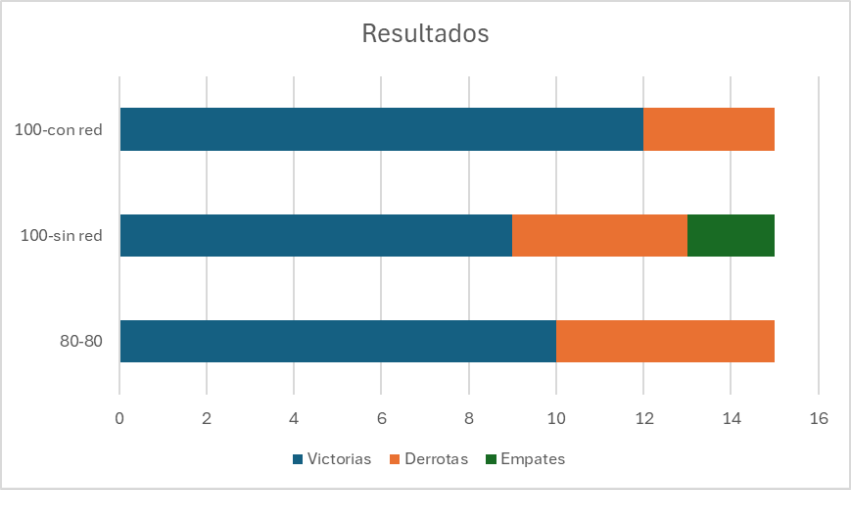
\includegraphics[width=0.45\textwidth]{grafico_resultados.png}
    \caption{Comparación de los resultados obtenidos.}
    \label{fig:resultados}
\end{figure}

Como es posible observar, la versión del agente con red neuronal que mejor resultados obtuvo fue la de cien iteraciones con doce victorias y tres derrotas. La versión de ochenta iteraciones sólo obtuvo diez victorias y cinco derrotas mientras que la versión de sólo cincuenta iteraciones empató dos veces con su adversario, además de lograr la victoria nueve veces y perder otras cuatro.

Adicionalmente, se analizó el balance de fichas en cada partida y se obtuvo lo mostrado en la figura~\ref{fig:balances}

\begin{figure}[htbp]
    \centering
    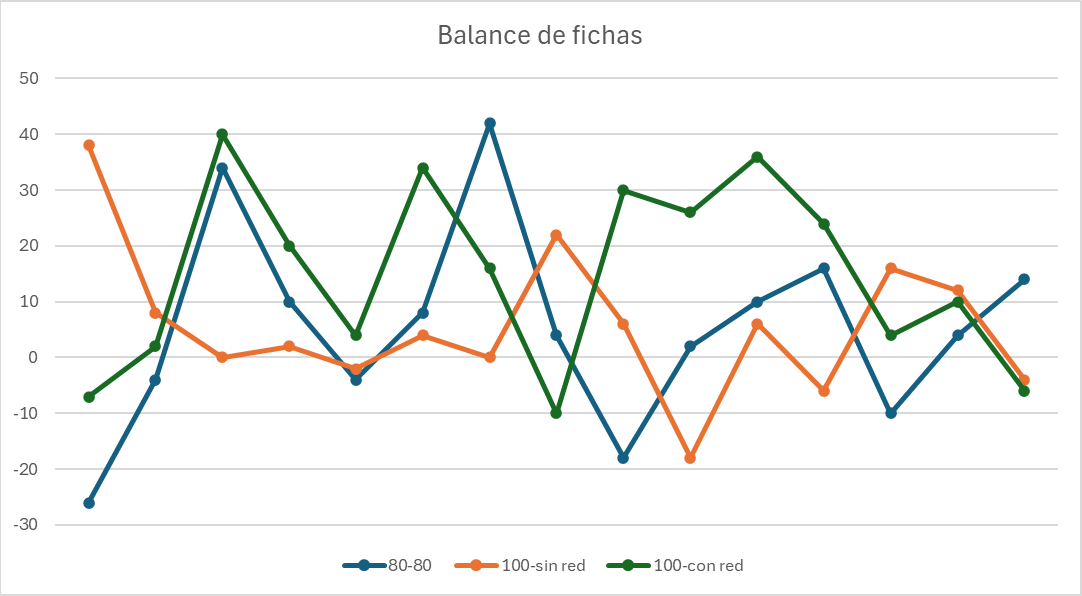
\includegraphics[width=0.45\textwidth]{grafico_balances.png}
    \caption{Comparación de los balances de las distintas partidas.}
    \label{fig:balances}
\end{figure}

El balance promedio que obtuvo el agente de cien iteraciones fue de \textbf{14,87} fichas, el de ochenta de \textbf{5,46} y el de cincuenta de \textbf{5,6}, todos en positivo. Podemos establecer una clara relación entre la efectivad del agente y: a) el número de iteraciones realizadas en el algoritmo MCTS, tanto para el agente que usa la red neuronal como para el agente que no la utiliza; b) el uso de la red neuronal a la hora de realizar las simulaciones en el algoritmo MCTS, en lugar de la elección aleatoria de movimientos.

Además de los resultados finales, debido a la posibilidad de poder observar los estados intermedios del tablero durante las cuarenta y cinco partidas jugadas en total, pudimos analizar (de manera superficial) tanto los movimientos realizados por los agentes como el tiempo que tardaron en hacer los movimientos. Por un lado, la tardanza en realizar los movimientos varió entre las distintas pruebas, siendo la siguiente para cada uno de los agentes:

\begin{itemize}
    \item \textbf{Agente MCTS sin red neuronal}
    \begin{itemize}
    	\item \textbf{100 iteraciones:} duración media de 59 milisegundos.
    	\item \textbf{80 iteraciones:} duración media de 30 milisegundos.
	\item \textbf{50 iteraciones:} duración media de 28 milisegundos.
    \end{itemize}
    \item \textbf{Agente MCTS con red neuronal}
    \begin{itemize}
    	\item \textbf{100 iteraciones:} duración media de 5,1 segundos.
    	\item \textbf{80 iteraciones:} duración media de 3,1 segundos.
	\item \textbf{50 iteraciones:} duración media de 1,42 segundos.
    \end{itemize}
\end{itemize}

(Estas mediciones se realizaron de manera manual y no se midieron todos los movimientos realizados de todas las partidas, sólo algunos de la mayoría de partidas que servirían como muestras representativas).

Por otro lado, fue posible detectar cuándo uno de los agentes no elegía el mejor movimiento a ojos de un humano (es decir, el movimiento que capturaría más fichas o un movimiento que no pondría en riesgo muchas de las fichas propias). Aunque esto no es algo realmente concluyente en este apartado de pruebas "IA contra IA", puesto que el mejor movimiento a los ojos de un humano no tiene por qué ser el mejor movimiento posible. Por ello, vimos necesario realizar las pruebas "IA contra humano" con el fin de averiguar si esos movimientos podían ser malas jugadas por parte de los agentes (malas jugadas de las que un humano sí se puede percatar) o buenas jugadas que fueron determinantes para la victoria del agente en cuestión y, por ende, el agente tenía un mayor dominio del juego de Otelo que una persona no experimentada en él (aunque tampoco desconocedora).

\subsection{Pruebas IA contra humano}
Para evaluar la efectividad del agente MCTS (con red neuronal) a la hora de enfrentarse a un humano se jugaron cinco partidas contra dicho agente. Cabe recalcar que el usuario que realizó las pruebas no fue en absoluto una persona experimentada en el juego de Otelo; aunque esta persona sí conocía las reglas de Otelo, sí había jugado anteriormente y múltiples veces contra sistemas ajenos a este trabajo y, supuestamente, más refinados y sí trataba de colocar fichas de la manera adecuada, sin realizar acciones al azar. En estas pruebas, el jugador humano usó las fichas negras y el agente las fichas blancas.

El resultado de las partidas fue de tres victorias para el humano y dos victorias para el agente. El balance de fichas (desde el punto de vista del humano) fue de -2, +26, -20, +16 y +34, es decir, una derrota ajustada, una derrota amplia y tres victorias también amplias.

\section{Conclusiones}
El algoritmo de Monte Carlo Tree Search es un algoritmo bastante eficiente para el desarrollo de agentes capaces de jugar a juegos de estrategia deterministas y conocidos como lo es el Otelo. Elige los movimientos a realizar en base a pruebas empíricas, pues las partidas simuladas que juega antes de tomar una decisión son partidas perfectamente realistas que sí pueden hacer ver que un movimiento es probable que lleve a una victoria o una derrota. Aunque no sólo eso, sino que hemos podido comprobar que es posible mejorarlo implementando una red neuronal para que el agente no se limite a realizar acciones aleatorias en las simulaciones y hemos sido capaces de ver su efectividad contra un agente que no hace uso de la mencionada red neuronal. A su vez, modificando las distintas iteraciones a realizar por ambos agentes, hemos comprobado que el agente de la red neuronal consigue un balance general de victorias positivo en todos los casos, siendo el más aplastante el de las cien iteraciones (mayor número de victorias y mejor balance general con catorce fichas, es decir, un promedio de victorias para nada ajustadas) y el menos eficiente el de sólo cincuenta iteraciones contra un agente que realiza cien, con algunos empates y un promedio de victorias ajustadas (sólo 5,6 fichas), aunque la balanza siguió inclinándose hacia el agente que hace uso de la red neuronal. 

Sin embargo, es necesario tener en cuenta que, por una parte, las partidas simuladas fueron escasas debido a la tardanza de las mismas. Sólo pudimos simular cuarenta y cinco partidas en total y somos conscientes de que es muy posible realizar las mismas pruebas y obtener resultados distintos. A pesar de ello, sí creemos que esas cuarenta y cinco partidas simuladas han sido suficientes para demostrar la mejora en la eficiencia que supone el uso de la red neuronal creada para las simulaciones que hace el algoritmo MCTS.

Por otra parte, no podemos obviar la tardanza del agente que hace uso de la red neuronal. El tiempo que implica usarla no es para nada despreciable, con una diferencia de uno, tres y hasta casi cinco segundos en el tiempo empleado en realizar una acción. Esto ha sido el principal motivo de la poca cantidad de partidas de prueba jugadas y creemos que es lo que hace que, a la vista de los resultados, se ponga en duda el uso de la red neuronal que hemos diseñado.

Aunque, por lo menos, podemos decir que el agente es capaz de jugar una partida contra un humano de manera eficiente, siendo capaz de ganar dos de cinco partidas jugadas.

En definitiva, aunque el uso de la red neuronal añade un coste computacional considerable, su integración en el agente MCTS ha demostrado ser una mejora efectiva en términos de rendimiento estratégico, sentando así una base sólida para futuras optimizaciones orientadas tanto a la velocidad como a la inteligencia del juego, especialmente a lo primero, pues es lo que más margen de mejora posee.

% ---------- Bibliografía ----------
\begin{thebibliography}{99}

\bibitem{russell2020}
S.~Russell and P.~Norvig, \emph{Artificial Intelligence: A Modern Approach}, 4th~ed. Pearson, 2020, ch.~5, ``Adversarial Search.''

\bibitem{browne2012}
C.~B.~Browne, E.~Powley, D.~Whitehouse, S.~M.~Lucas, P.~I.~Cowling, P.~Rohlfshagen, S.~Tavener, D.~Perez, S.~Samothrakis, and S.~Colton, ``A survey of Monte Carlo tree search methods,'' \emph{IEEE Transactions on Computational Intelligence and AI in Games}, vol.~4, no.~1, pp.~1--43, 2012. [Online]. Available: \url{https://ieeexplore.ieee.org/document/6145622}

\end{thebibliography}


% ---------- Fin del documento ----------
\end{document}